\documentclass[a4paper]{article}
\usepackage{polski}
\usepackage[utf8]{inputenc}
\usepackage{enumerate}
\usepackage{hyperref}
\usepackage{graphicx}
\usepackage{float}
\usepackage{geometry}
\usepackage{verbatim}

\title{Wizualizacja danych sensorycznych - projekt}
\date{}

\begin{document}
\maketitle

\begin{enumerate}

\item Temat projektu:

Wizualizacja pogody w Japonii.

\item Wykonawca:

Filip Malinowski 209193

\item Opis projektu:

Projektowany program będzie pobierać pogodę z internetowych serwisów pogodowych. Dane będzie aktualizował dynamicznie co okres czasu wybrany przez użytkownika, np. co 1 minutę, 1 godzinę, 2 godziny. Informacje o pogodzie będą wyświetlane na mapie.

Interaktywność mapy będzie polegać na tym, że domyślnie dla każdej stolicy prefektury będzie wyświetlana temperatura i ikona zachmurzenia. Po najechaniu kursorem na nazwę miasta rozwinie się szczegółowa pogoda zawierająca: temperaturę, szansę opadów, ciśnienie, wilgotność, zachmurzenie, prędkość i kierunek wiatru oraz poziom promieniowania UV.

W programie będzie również druga zakładka, w której użytkownik będzie mógł wyszukać miasto i wyświetlić dla niego szczegółowe informacje na temat pogody. Wyświetlona zostanie prognoza godzinowa wszystkich czynników podanych wcześniej do wyświetlania na mapie oraz odpowiednie wykresy.

Ma być też możliwość dodania nowych zakładek za pomocą zakładki +. Wtedy jej konfiguracja będzie przebiegać tak samo jak dla drugiej zakładki. Schemat jej zawartości będzie taki sam jak w przypadku drugiej zakładki. Dodatkowe zakładki będą umożliwiać skasowanie się.

\item Źródła pogodowe:
Dane pogodowe są pobierane z serwisu developer.forecast.io. Serwis ten pozwala na 1000 darmowych zapytań dziennie ale przy tym udostępniając bardzo dużo danych pogodowych. Dane z tego serwisu pochodzą z: USA NOAA’s NEXRAD system, UK Met Office’s NIMROD system, The USA NOAA’s LAMP system, UK Met Office’s Datapoint API, Norwegian Meteorological Institute’s meteorological forecast API, USA NOAA’s Global Forecast System, USA NOAA’s Integrated Surface Database, USA NOAA’s Public Alert system, UK Met Office’s Severe Weather Warning system, Environment Canada’s Canadian Meteorological Center ensemble model, US Navy’s Fleet Numerical Meteorology and Oceanography Ensemble Forecast System, USA NOAA and Environment Canada’s North American Ensemble Forecast System, USA NOAA’s North American Mesoscale Model, USA NOAA’s Rapid Refresh Model, Norwegian Meteorological Institute’s GRIB file forecast for Central Europe, Norwegian Meteorological Institute’s GRIB file forecast for Northern Europe, Worldwide METAR weather reports, USA NOAA/NCEP’s Short-Range Ensemble Forecast, USA NOAA/NCEP’s Real-Time Mesoscale Analysis model, USA NOAA/ESRL’s Meteorological Assimilation Data Ingest System.

Dane ze wszystkich powyżej wymienionych serwisów są następnie uśredniane i przesyłane do użytkownika na zapytanie wysłane do developer.forecast.io. Serwis ten korzysta z bezpiecznego połączenia szyfrowanego protokołem SSLv2.


\item Zrealizowane funkcjonalności:
\begin{itemize}
\item Widżet Mapa z mapą Japonii jako tło;
\item Obiekt Miasto pobierający i przechowujący dane pogodowe;
\item Zakładka przechowująca obiekt klasy Miasto i wyświetlająca wykresy;
\item Obiekt wyszukujący koordynaty miasta na podstawie podanej nazwy.
\end{itemize}

\item Funkcjonalności do zrealizowania:
\begin{itemize}
\item Chmurki umieszczone na mapie wyświetlające ikonę pogody oraz temperaturę;
\item Belka z ustawieniami dająca możliwość ustawienia okresu odświeżania danych.
\end{itemize}

\item Opis zaimplementowanych funkcjonalności:
\begin{itemize}

\item Widżet Mapa
Przechowuje plik png z mapą Japonii oraz wskaźnik na obiekt klasy QLabel. Wykorzystuje obiekt QLabel w celu ustawienia swojego tła jako mapę Japonii. Widżet ten jest skaluje się wraz ze zmianą rozmiaru całego okna.

Docelowo na mapie mają być wyświetlane chmurki przy większych miastach Japonii pokazujące temperaturę i ikonę zachmurzenia w tych miejscach. Po najechaniu na ikonę miasta chmurka ma się rozwinąć przedstawiając szczegółowe informacje nt tego miejsca.

\item Obiekt Miasto
Obiekt ten modeluje jedno miasto. Przechowuje koordynaty miasta oraz dane pogodowe na temat tego miasta w formacie json. Łączy się z serwisem internetowym developer.forecast.io pobierając z niego dane pogodowe. Następnie konwertuje odebrane dane do formatu obsługiwanego przez klasę składową obiektu Miasto, QJsonObject.
W obiekcie Miasto są metody umożliwiające dostęp do fragmentów klasy QJsonObject wycinając z niego opis pogody, dane pogodowe, itp.

\item Widżet OknoZZakladkami
Widżet ten modeluje fragment głównego okna programu będący widżetem z zakładkami. Ma możliwość zmiany swojego rozmiaru wraz ze zmianą rozmiaru głównego okna programu. Tworzy się z dwiema zakładkami: mapą oraz zakładką miasta, która wyświetla informacje pogodowe dla Tokio.

Docelowo zakładka miasta wyświetli zapytanie o nazwę miasta w celu wyświetlenia danych pogodowych. Wyszukane propozycje miast wyświetlą się w ComboBox. Będzie jeszcze trzecia zakładka ze znakiem + dodająca kolejne zakładki z miastami. Po dodaniu nowej zakładki z miastem trzeba będzie ustawić miasto tej zakładki. Po tym zostaną pobrane informacje. Skasować będzie można tylko dodane zakładki. Dwóch pierwszych nie będzie dało się skasować. Ilość zakładek w sumie nie będzie mogła być większa niż 5.

\item Widżet ZakladkaMiasta
Widżet ten wyświetla aktualną temperaturę, ciśnienie i wilgotność w pierwszym rzędzie. W drugim rzędzie wyświetla wykres zmiany temperatury w przeciągu 48 godzin. W trzecim rzędzie wyświetla wykres zmiany temperatury w przeciągu 7 dni.

\item Obiekt WyszukiwarkaMiasta
Obiekt ten wyszukuje koordynaty miasta na podstawie podanej nazwy. Informacje wyszukuje w serwisie Here firmy Nokia.

\end{itemize}

\pagebreak
\item Opis funkcjonalności do implementacji:
\begin{itemize}
\item Aktualizacja widżetu Mapa
Za pomocą paintEvent na mapie mają być wyrysowane temperatury dla odpowiednich regionów Japonii. Tło również ma zostać wyrysowane z pliku z mapą Japonii.

\item Połączenie obiektu Miasto z obiektem WyszukiwarkaMiasta
Skorzystanie z obiektu WyszukiwarkaMiasta w obiekcie Miasto w celu otrzymania możliwości wysuzkiwania miasta na podstawie nazwy, nie koordynatów. Wyszukiwarka miasta szuka koordynatów na podstawie szukanego słowa, a obiekt miasto za pomocą koordynatów pobiera dane pogodowe.
\end{itemize}

\item Harmonogram:

\begin{description}
\item[9 kwietnia - zrealizowane] | przeprowadzenie badań na temat najlepszych źródeł informacji oraz odpowiedniej struktury programu;

\item[22 kwietnia - zrealizowane] | napisanie wersji alpha programu realizującej podstawowe funkcje programu. Podstawowymi funkcjami do realizacji są: wyświetlenie mapy Japonii, pobranie danych z serwisów pogodowych i zapisanie ich w klasie danego miasta;

\item[23 kwietnia - zrealizowane] | podsumowanie wstępnej wersji programu oraz ewentualne poprawki w planach projektu;

\item[29 kwietnia - zrealizowane] | przekazanie wstępnej wersji programu do oceny;

\item[6 maja - zrealizowane] | dodanie dwóch kolejnych funkcjonalności: zakładki z obiektem Miasto oraz wyszukiwanie koordynatów miasta na podstawie podanej nazwy;

\item[20 maja - w trakcie] | połączenie działania wyszukiwarki miasta z obiektem Miasto oraz wyrysowanie temperatur na mapie Japonii w pierwszej zakładce.
\end{description}

\pagebreak
\item Diagram przepływu sterowania:\\
\begin{figure}[H]
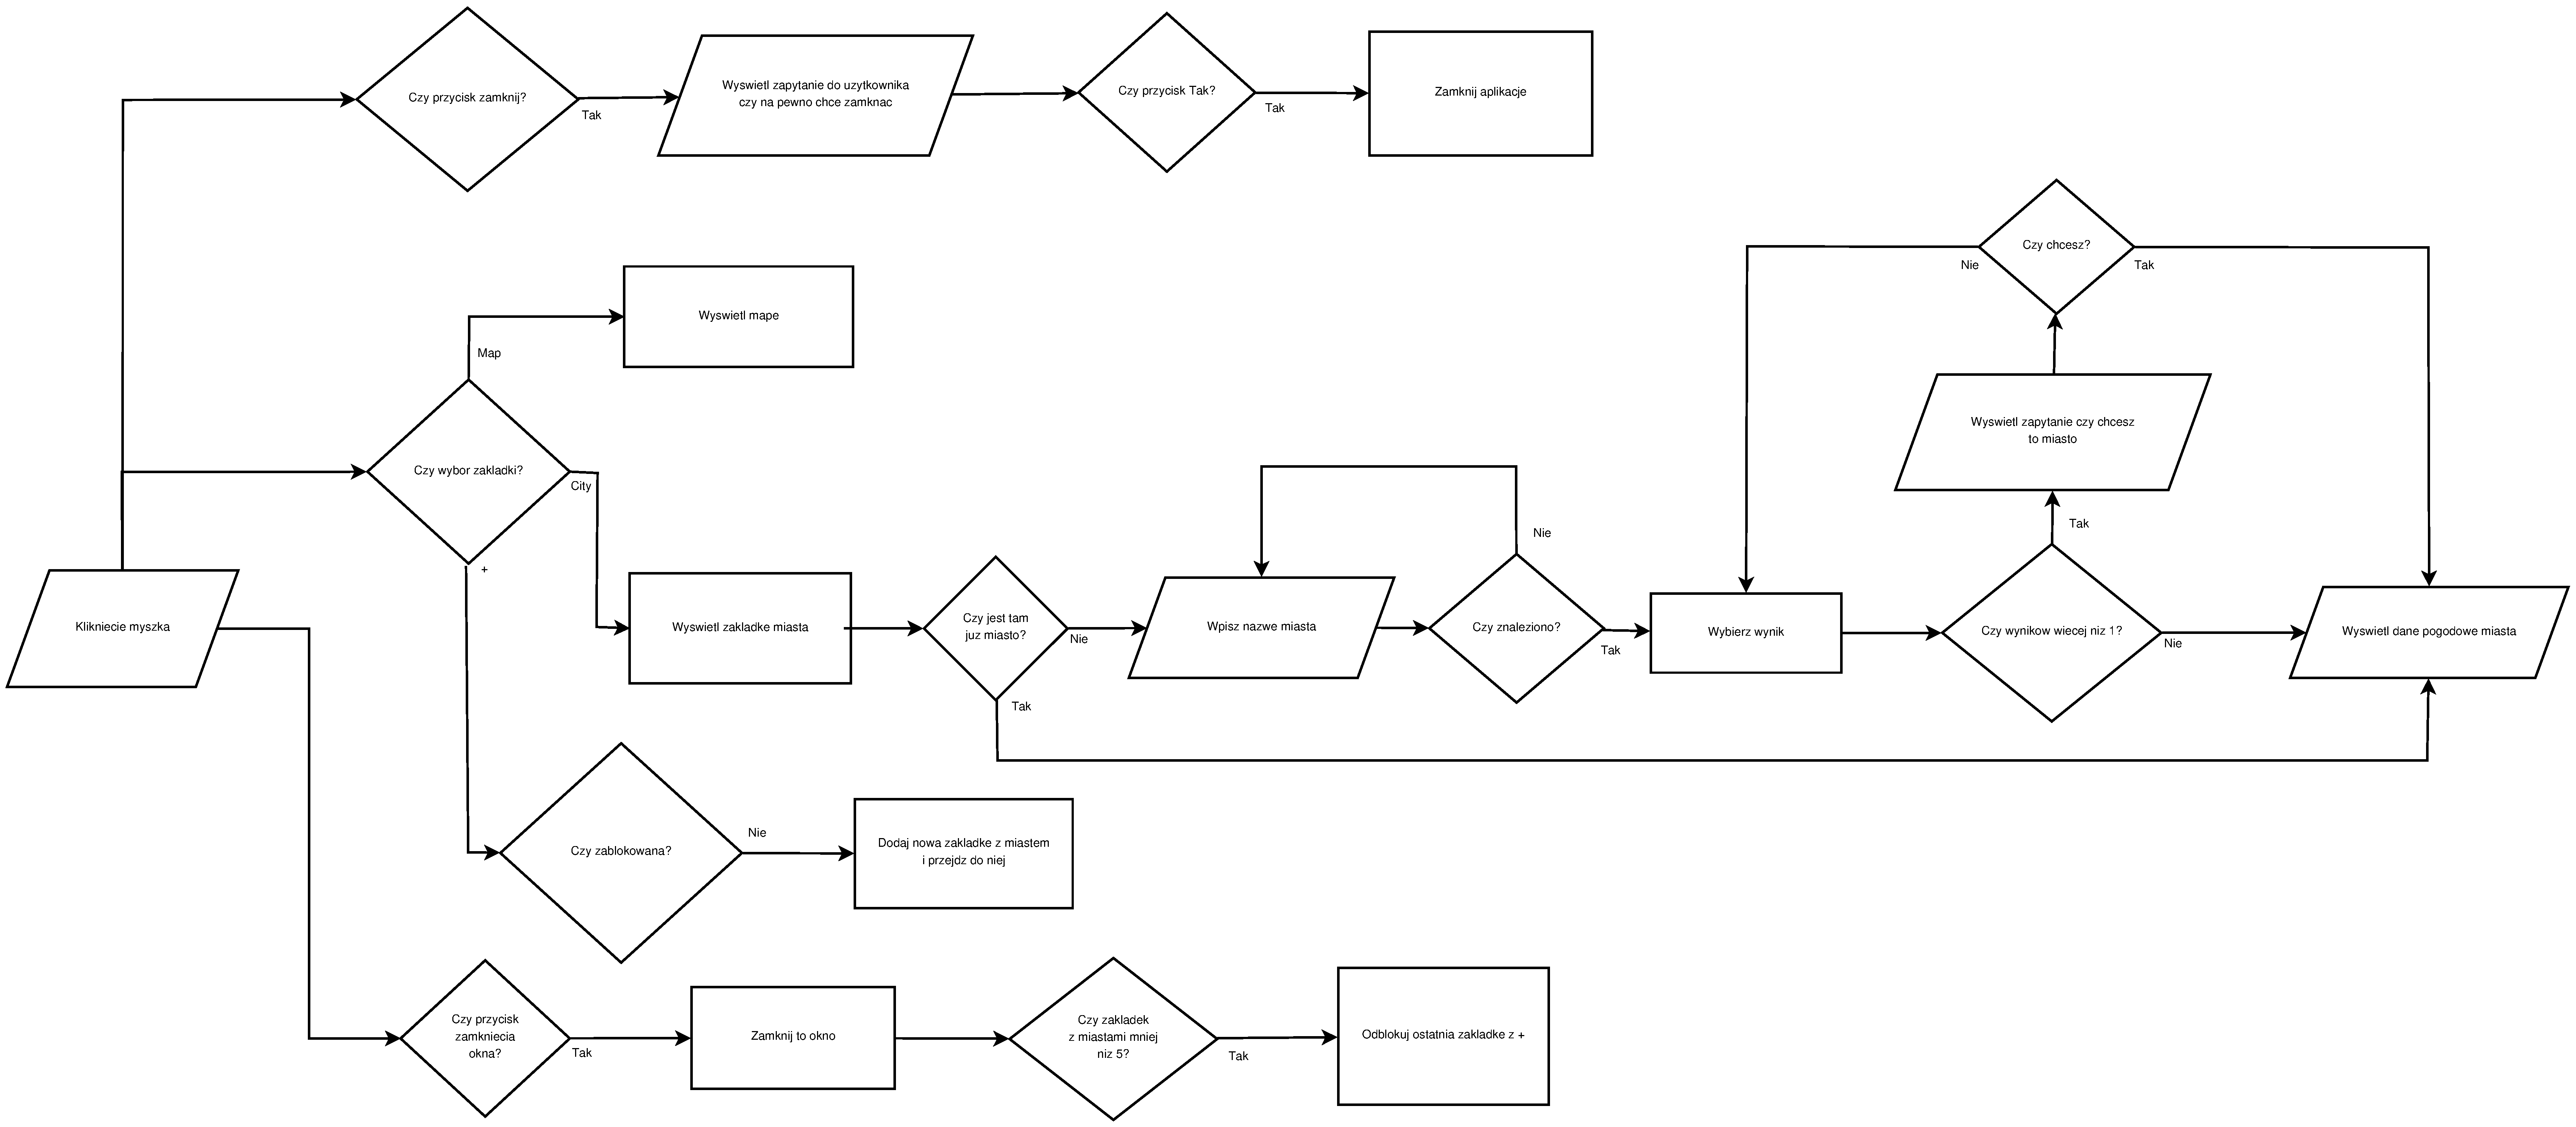
\includegraphics[width=15cm]{przeplyw.eps}
\end{figure}

\pagebreak
\item Diagram klas:\\
\begin{figure}[H]
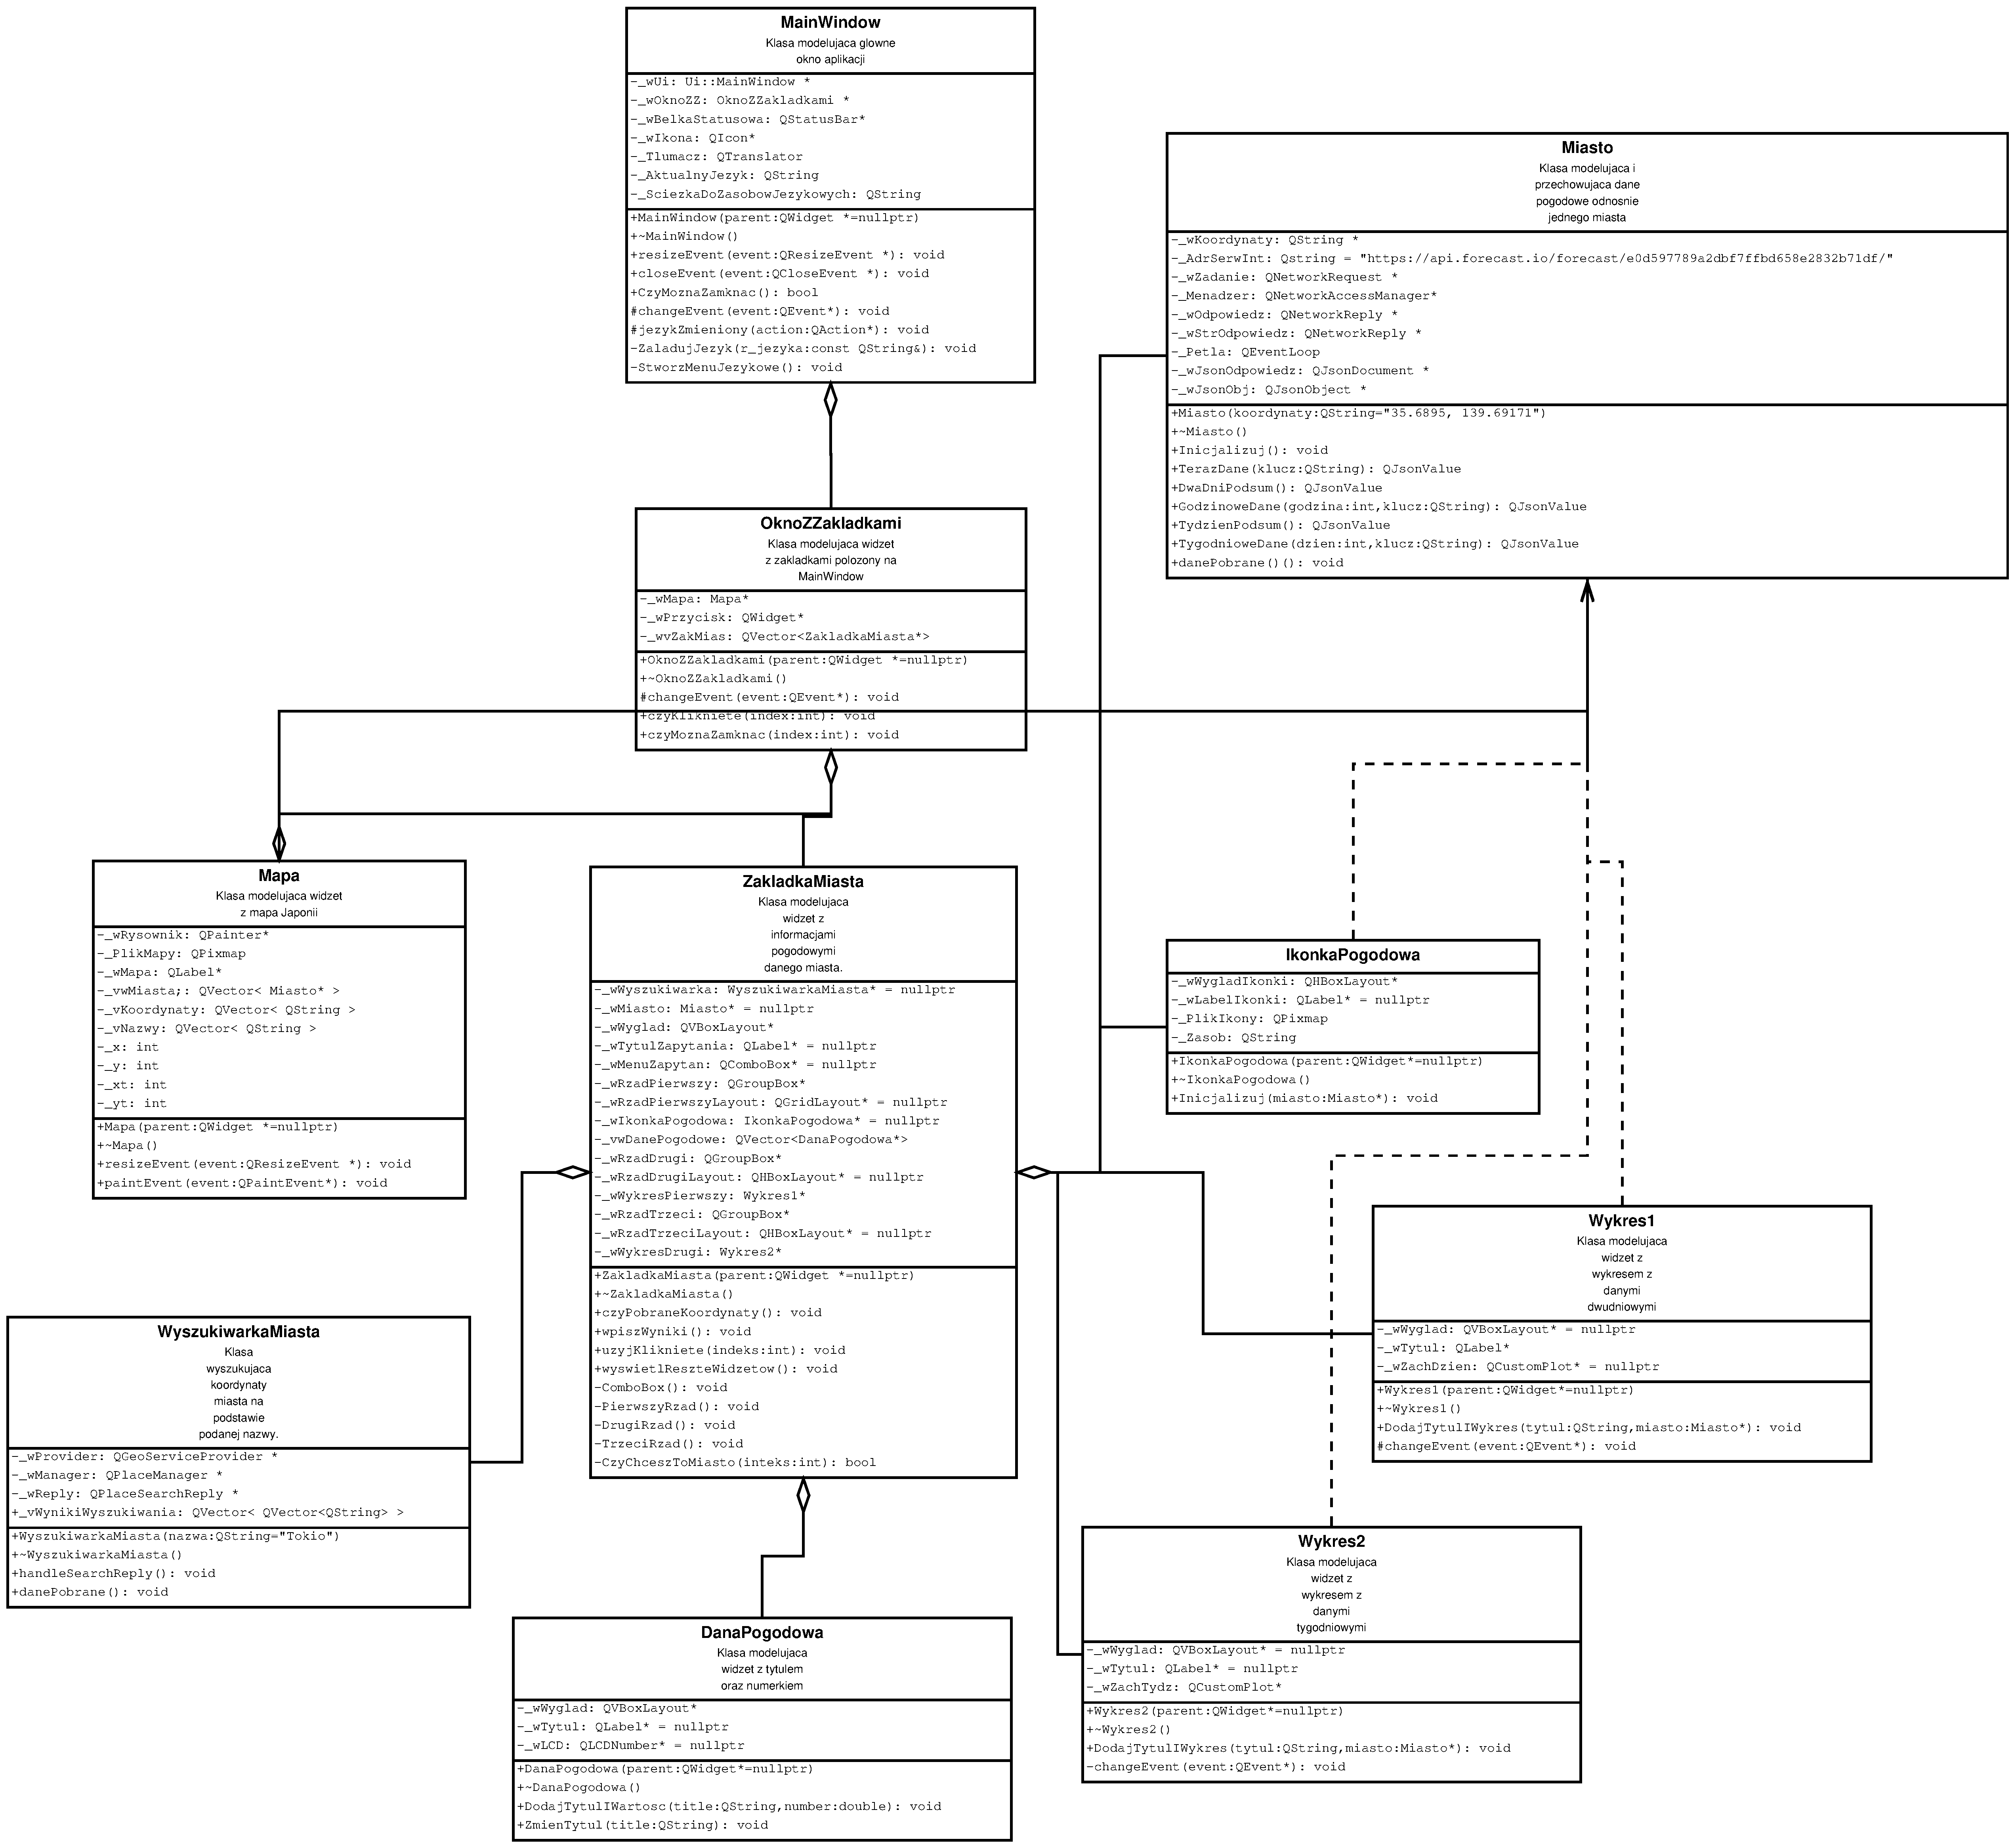
\includegraphics[width=14cm]{diagram_klas.eps}
\end{figure}

\begin{comment}
\pagebreak
\item Layout zakładki mapa:\\
\begin{figure}
\includegraphics[bb=0 0 600 400]{proponowany_layout_mapa.png}
\end{figure}

\pagebreak
\item Layout zakładki miasto:\\
\begin{figure}
\includegraphics[bb=0 0 600 400]{proponowany_layout_miasto.png}
\end{figure}
\end{comment}

\item Zarządzanie projektem:
\begin{itemize}
\item Git - do przechowywania i rozwijania dokumentacji oraz oprogramowania związanego z projektem.
\href{https://github.com/hizonglol/wds-2016}{Adres internetowy repozytorium.}
\item LaTeX - do tworzenia dokumentacji projektu
\end{itemize}
\end{enumerate}
\end{document}